\documentclass[11pt]{article}
\usepackage{hyperref}
\usepackage{graphicx}
\usepackage{float}
\usepackage{geometry}

\geometry{
a4paper,
total={170mm,257mm},
left=20mm,
top=20mm,
}
\hypersetup{
    colorlinks=true,
    linkcolor=blue,
    filecolor=magenta,      
    urlcolor=cyan,
}

\title{Analyzing Patterns of Computational Similarity between Protein Kinase Ligands}
\author{Jack Ringer}
\date{July 2025}


\begin{document}

\maketitle


\section*{Abstract}
This work investigates whether there is a relationship between the 2D computational similarity of ligands and their activity within specific human protein kinase groups.  
Using data from ChEMBL binding assays, the distribution of pairwise Tanimoto similarity coefficients values computed between all kinase ligands was compared against the distribution of pairwise similarity values computed with respect to ligands active within a specific kinase group. 
With the exception of the CK1 group, no significant group-specific differences were found. 
These results suggest there is limited utility of 2D similarity metrics for identifying ligand selectivity across a majority of kinase groups. 
However, given the many confounders that exist when performing large scale computational analyses of ChEMBL bioassay data these results are not definitive, and limitations as well as potential follow-ups are discussed in detail. 
All code developed as part of this project can be found on GitHub: \href{https://github.com/Jack-42/ligandActivityAnalysis}{https://github.com/Jack-42/ligandActivityAnalysis}. 

\section*{Introduction and Background}
This work explores the relationship between 2D ligand similarity and the activity of these ligands with respect to major protein kinase families. 
The following sections provide a brief overview of protein kinases and their classification, molecular similarity, the project's relevance to drug discovery, and related works.


\subsection*{Protein Kinases}
Given their (nearly impossible-to-overstate) importance in drug discovery, medicine, and biology + chemistry broadly, an immense amount of effort has been put into classifying proteins. 
One of the most significant protein families studied by drug discovery researchers is the protein kinase family. 
These protein kinases (PKs) are enzymes which modify the function of other proteins via phosophorylation~\cite{lubos_cipak_2022}. 
PKs are involved in many important regulatory roles throughout the cell, and their dyregulation is linked to many types of cancer as well as immune, neurological and infectious diseases~\cite{cancer as well as immune, neurological and infectious diseases}. 
Although all PKs perform phosophorylation, they do not all perform the same function (e.g., some PKs will target different protein domains than others). 

One of the first kinase classifications was published by Manning and other researchers in 2002~\cite{manning_2002}. 
Their research has resulted in the establishment of 8 major groups within the human kinome, which include: AGC, CAMK, CK1, CMGC, STE, TK, TKL, Other, as well as 13 atypical families~\cite{eid_turk_volkamer_rippmann_fulle_2017}.
Generally speaking, these groups (as well as the families and subfamilies they contain) have been classified based on sequence similarity, evolutionary conservation, and known functions. The exception to this is the ``Atypical'' and ``Other'' groups, which serve to classify proteins which don't fit into the other major groups. 
A phylogenetic tree of the human kinome is shown in Figure~\ref{fig:fam_tree}. % TODO: maybe rephrase here

\begin{figure}[H]
    \centering
    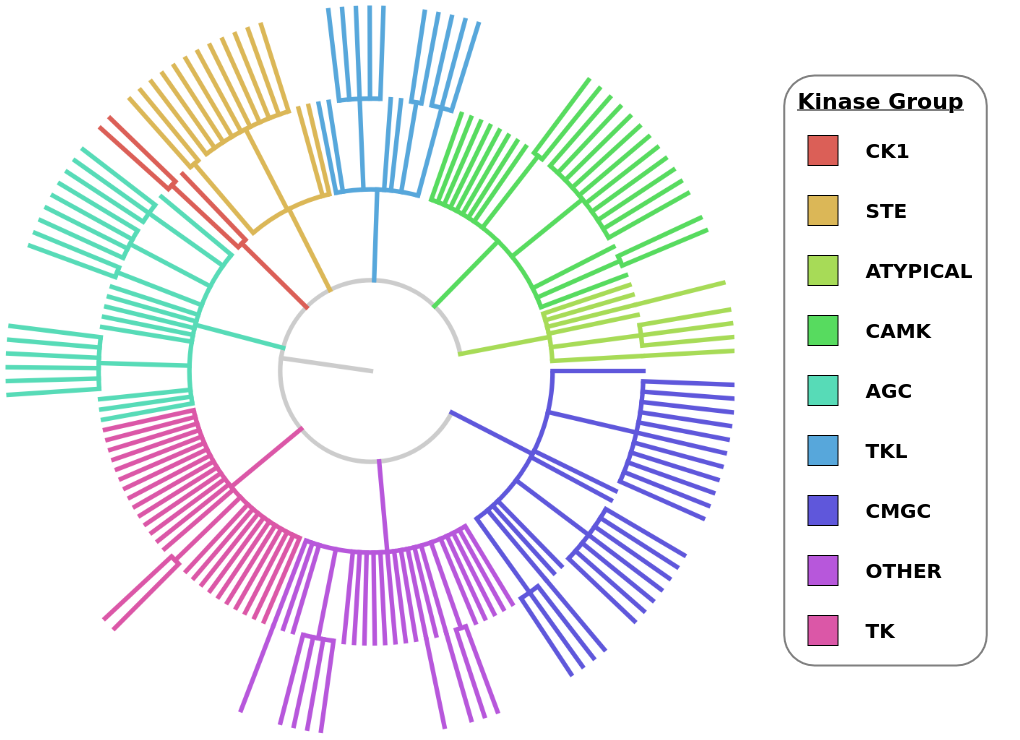
\includegraphics[width=0.7\textwidth]{../figures/protein_family_tree.png}
    \caption{Phylogenetic Tree of the Human Kinome showing major groups as well as families and subfamilies. Generated using ETE4 with data from CheMBL.}
    \label{fig:fam_tree}
\end{figure}


\subsection*{Molecular Similarity}
The similarity property principle (SPP), has been enormously influential in the realm of medicinal chemistry~\cite{maggiora_vogt_stumpfe_bajorath_2013}. 
According to the SPP, structurally-similar compounds often exhibit similar properties. 
Among these properties is biological activity, such that similar compounds often demonstrate similar activity against identical biological targets (i.e., proteins in a majority of cases). 
It is important to note that the definition of ``similar'' here is ambiguous, and can be measured in a myriad of ways. 
Additionally, there exist so-called ``activity cliffs'', where a compound which shows high binding affinity (i.e., high activity) against a given target becomes completely ineffective after minor structural modifications~\cite{maggiora_vogt_stumpfe_bajorath_2013,filip_miljkovic_jurgen_bajorath_2018}.  


There are many computational methods for computing molecular similarity between two compounds [4]. Similarity calculations depend both on how compounds are represented (e.g., using molecular graphs, fingerprint vectors, etc), as well as the particular metric used. These similarity metrics typically report a value in the range 0 to 1, with values closer to 1 indicating a higher degree of structural similarity. In addition to computing pairwise similarity, dimensionality-reduction methods (e.g., U-MAP) can be used with clustering algorithms (e.g., K-means) to group together multiple structurally-similar compounds. Other clustering approaches make use of molecular scaffolds or other well-defined structural motifs.

For the purposes of this project... % TODO: tanimoto coeff explanation

\subsection*{Relevance to Drug Discovery}
% With few exceptions, for a drug to produce an effect it must bind to specific components of cells and tissues~\cite{antolin_ameratunga_banerji_clarke_workman_al-lazikani_2020}. 
% These biological targets are most commonly proteins, although they can also include nucleic acids and peptides~\cite{gashaw_ellinghaus_sommer_asadullah_2011}.  
% A molecule which is ``active'' (as measured by, for example, an IC50 value) against a given disease-related target may be a promising drug candidate. 
% In the case of protein kinases, these drug candidates are often identified from binding assays which measure whether or not the molecules
% TODO: probably need to rephrase above

As mentioned above, protein kinases are involved in a number of human pathologies. 
If there is a relationship between protein kinase group and ligand similarity, then it may be informative to look at the ligands of related kinases (i.e., those belonging to the same group). 
This would be especially beneficial if there are few known ligands for the target of interest, as one could leverage data from well-studied, closely-related proteins to inform the discovery process. 

\subsection*{Related Works}
The idea that similar compounds may exhibit similar activities against proteins within the same family (or group) is not new. 
The term ``intrafamily polypharmacology'' (IFP) refers to molecules which have demonstrated activity against multiple proteins belonging to the same family, and has been of special interest in (for instance) studying PARP-1 inhibitors~\cite{passeri_camaioni_liscio_sabbatini_ferri_carotti_giacchè_pellicciari_gioiello_macchiarulo_2015, antolin_ameratunga_banerji_clarke_workman_al-lazikani_2020}. 
Relatedly, previous works have investigated the theory of ``Target-Family-Privileged Substructures'', which suggests that particular chemical substructures are strongly linked to activity against certain protein families~\cite{schnur_hermsmeier_tebben_2006}. 
Several works have developed computational analyses for looking at activity relationships between families~\cite{bajorath_2008}, and works such as \cite{filip_miljkovic_jurgen_bajorath_2018} and \cite{lo_liu_morrissey_kakiuchi-kiyota_johnson_broccatelli_zhong_joshi_altman_2018} have investigated the structures and activities of kinase inhibitors. 


\section*{Methodology}\label{sec:methodology}

\section*{Results}
\subsection*{Distribution}

Figure~\ref{violin_plot} provides distributions for the ${N\choose 2}$ similarity values per group ($N$ = number of ligands), as well as the ${9,995 \choose 2} = 49,945,015$ similarity values calcualted for all kinase ligands in the dataset. Table~\ref{results_table} provides additional statistics for each group, as well as results from a Mann-Whitney U test (MWUT).
\begin{figure}[H]
    \centering
    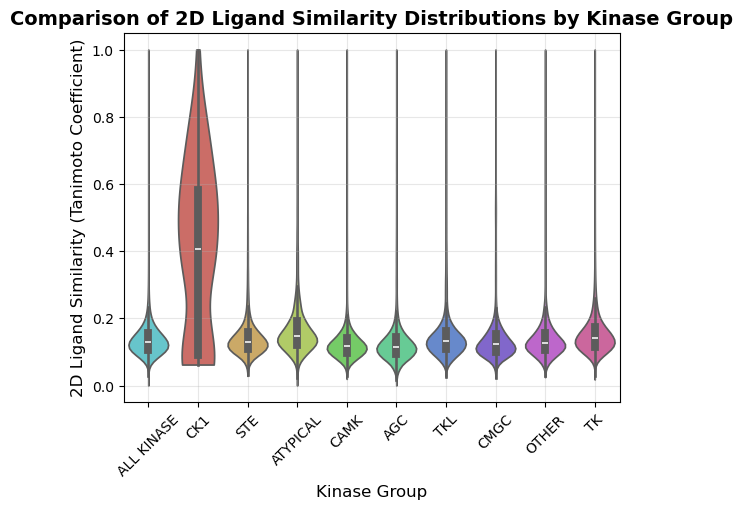
\includegraphics[width=0.75\textwidth]{../figures/violin_plot.png}
    \caption{Comparison of 2D structural similarity distributions by kinase group}
    \label{violin_plot}
\end{figure}

\begin{table}[!ht]
\centering
\resizebox{\textwidth}{!}{\begin{tabular}{|l|l|l|l|l|l|}
    \hline
    \textbf{Kinase Group} & \textbf{N. Targets} & \textbf{N. Ligands} & \textbf{Group Median} &\textbf{Comparison Median} & \textbf{MWUT p-value} \\ \hline
    CK1 & 10 & 13 & 0.407 & 0.129 & $3.10 \times 10^{-11}$ \\ \hline
    STE & 45 & 425 & 0.131 & 0.129 & $2.48 \times 10^{-169}$ \\ \hline
    ATYPICAL & 15 & 357 & 0.149 & 0.129 & $< 5 \times 10^{-324}$ \\ \hline
    CAMK & 65 & 597 & 0.117 & 0.130 & $1.0$ \\ \hline
    AGC & 59 & 809 & 0.116 & 0.131 & $1.0$ \\ \hline
    TKL & 37 & 810 & 0.133 & 0.129 & $< 5 \times 10^{-324}$ \\ \hline
    CMGC & 58 & 1275 & 0.122 & 0.130 & $1.0$ \\ \hline
    OTHER & 56 & 727 & 0.127 & 0.129 & $1.0$ \\ \hline
    TK & 80 & 5347 & 0.140 & 0.121 & $< 5 \times 10^{-324}$ \\ \hline
\end{tabular}}
\caption{Table showing comparisons of targets, ligands, and ligand similarity distributions per kinase group. Shown p-values are calculated (with Bonferroni correction) from a MWUT where the alternative hypothesis is that the similarity values within the group are stochastically greater than the distribution of all similarity values.}\label{results_table}
\end{table}



\subsection*{Enrichment}

\section*{Discussion}
% include limitations here

\section*{Conclusion}


\section*{Acknowledgement}
Much thanks to my advisor Dr.~Vincent Metzger for his guidance and input over the course of this project. I'd also like to thank Dr.~Jeremy Yang, Dr.~Cristian Bologa, and Dr.~Praveen Kumar for their feedback during weekly meetings over the course of the internship. Finally, I'd like to thank the   authors of ChEMBL DB~\cite{chembl_db_2023}.

\bibliographystyle{plain}\bibliography{report}

\end{document}
